\section{Scaling across arbitrary number of Nodes}

The previously discussed Master-Worker algorithms expect all the data before and after a contraction to reside within 1 node.
For large tensors this is no longer feasable, as scratch memory on a node is limited and using main storage is prohibitively slow.
The communication load is also very unbalanced for more than 2 nodes, where the master has to communicate with all other nodes while each node only has to communicate with the master.
To circumvent all these problems the next algorithms will keep the data distributed in the whole contraction.
This needs both less memory on each node and allows very balanced communication loads.

As basis for the following algorithms we make a few assumptions:
\begin{enumerate}
    \item tensors are predistributed across all nodes 
    \item gathering the result tensor is not needed
    \item tensors are sufficiently large and compute intensive that data communication will not be the bottle neck
    \item tensors can be split evenly across ranks
\end{enumerate}

To justify point 1 and 2 we consider our examples as part of a larger Einsumtree that gets contracted.
If the tree is large enough, the initial distribution and the final gatherering of tensors will be negligble compared to the total runtime.
If point 3 is not met the tree should be run on less nodes.
If the tree is sufficiently small just one node and no distributed memory parallelism whatsoever might be better suited towards the problem.
Point 4 is assumed so the algorithms can be described in a simpler manner.
If the system proposed is to be deployed as more than just this proof of concept, one could remedy that requirement by zero padding input tensors or adjusting the algorithms to work on two sizes of each tensor instead (one for the fully filled chunks and one for the partial chunks).

With these assumptions met the main goal for the algorithms will be to increase throughput as much as possible.
To achieve that each node has to compute ideally the entire runtime of a contraction, which necessitates overlapping communication and computation (should communication occur).
The following algorithms will employ an extra communication thread to achieve this overlap.
This work proposes 3 algorithms for the following scenarios:
\begin{enumerate}
    \item in both input tensors the same c dimension is split
    \item in both input tensors a m/n dimension is split
    \item in both input tensors the same k dimension is split and one tensors outer most dimension is m/n
\end{enumerate}

\subsection{distributed c dimension algorithm}

\begin{figure}[h]
\centering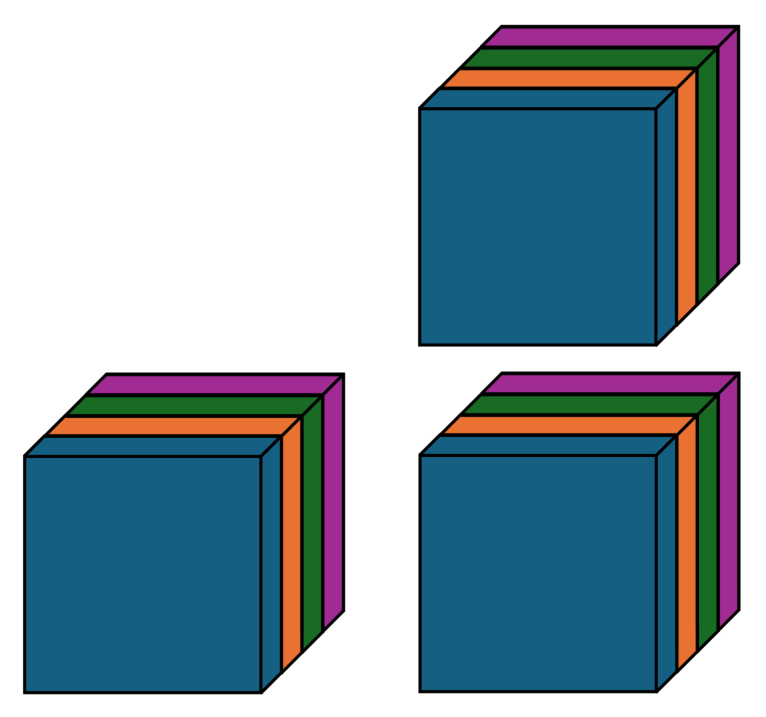
\includegraphics[width=0.3\textwidth]{dist_c.pdf}
\caption{Visualization of the distributed c algorithm; 
each color represents one node with the coloured blocks representing the data they hold; 
since the tensors are distributed along their c dimension, each node can locally contract its chunks to generate their chunk of the output tensor}
\label{fig:c_algo}
\end{figure}

Distribution along a c dimension is the simplest algorithm we consider. 
As seen in Figure \ref{fig:c_algo} we assume both input tensors are distributed along the same c dimension.
We also generally expect all distributions to follow the same order within ranks, meaning that rank 0 always keeps the first chunk, rank 1 the second and so on.
If now both input chunks are contracted on each node, the result will be a chunk of the output tensor distributed along the same c dimension.
At least locally this is optimal, since all nodes have the same workload and no additional communication has to occur.
As long as a tensor can be split among all nodes, this algorithm is preferable to the non distributed case.

\subsection{distributed m/n dimensions algorithm}

\begin{figure}[h]
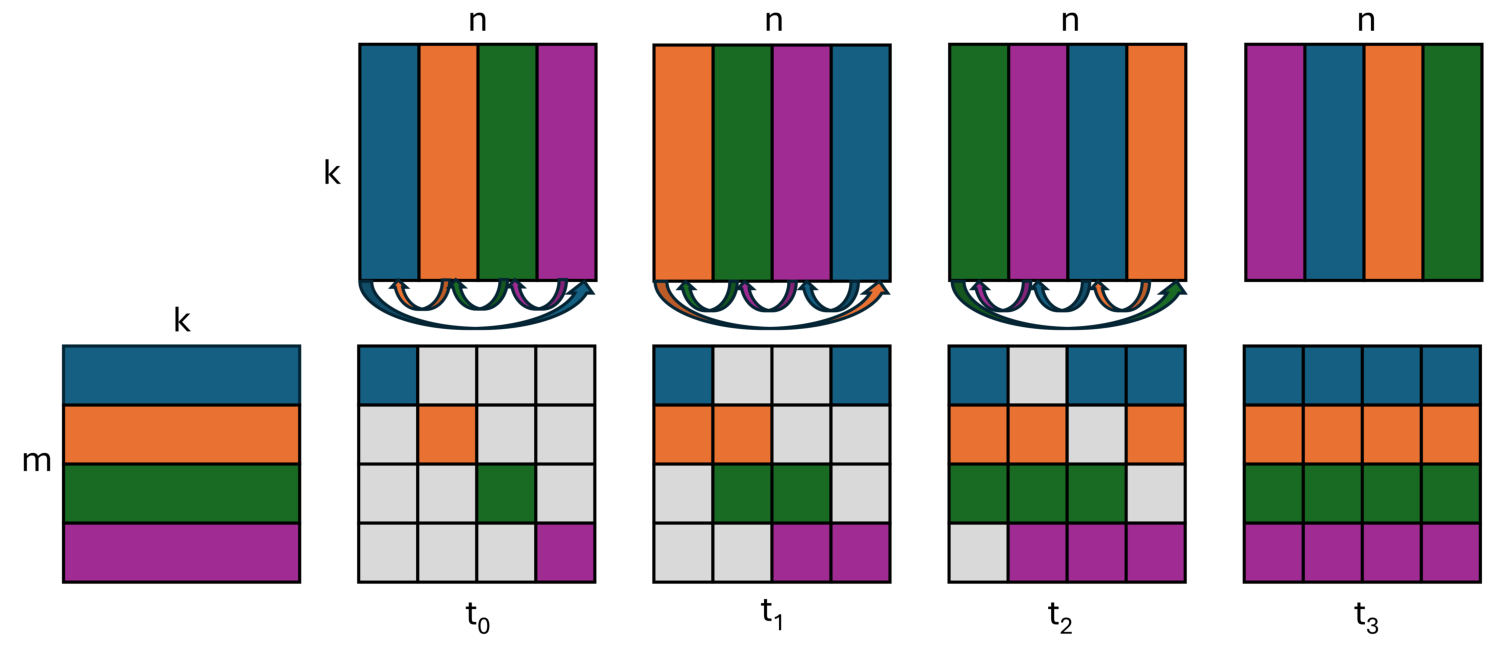
\includegraphics[width=0.78\textwidth]{dist_m_n_out_m.pdf}
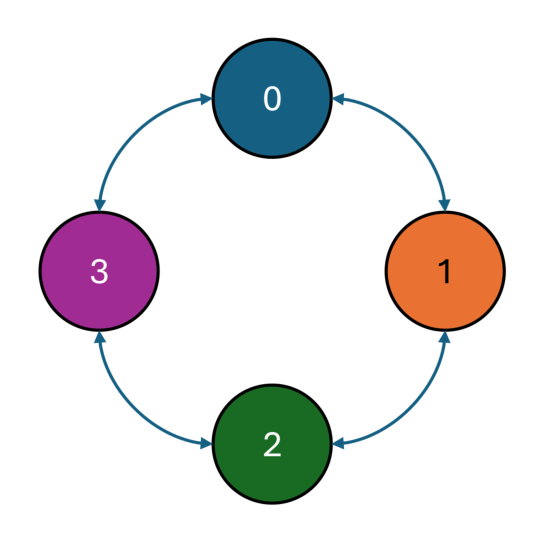
\includegraphics[width=0.2\textwidth]{ring.pdf}
\caption{Visualization of the distributed m/n algorithm; 
each color represents one node with the coloured blocks representing the data they hold; 
since the tensors are split along their m/n dimensions each node can only locally contract $\frac{1}{totalNodes}$th part of the output tensor.
To generate a full chunk of the output tensor, each node contracts its current right tensor with their left tensor while simultaneously sending it to their previous neighbour in the ring and receiving their next right tensor from their next neighbour.
In the visualization this is described with arrows originating on the communicated chunk and coloured with its recipient.
The ring communication used is depicted on the right, where each node can only communicate with its immediate neighbours.
After $totalNodes$ steps this will result in an output tensor that is distributed along the same dimension as the left tensor.
}
\label{fig:m_n_algo}
\end{figure}

For the communication of this algorithm we assume that all nodes are set up in a ring as seen in the right part of Figure \ref{fig:m_n_algo}.
If both input tensors are distributed alongside their m/n dimensions, communication between nodes is unavoidable.
In contrast to being distributed along their c dimension, each node can only calculate a $\frac{1}{n^2}$ big chunk of the output tensor locally, where n is the number of nodes employed in the distributed contraction.
Each node needs to end up with a $\frac{1}{n}$ big chunk of the output tensor.
This algorithm achieves this by doing $n$ contractions, where the first $n-1$ contractions are overlapped by each node communicating its currently being contracted right tensor to the previous node in the ring.
In each step $\frac{1}{n}$'th of each nodes chunk of the output tensor is calculated.
Due to a limitation in the contraction interface of the current application, the outer most dimension of the output tensor has to be the distributed dimension of the right tensor, as the interface expects input and output tensors to be contiguous in memory.
This limitation could be circumvented by inputting not just the tensors but also their strides into the interface.
In the rest of this thesis that limitation will be disregarded.
This algorithm only has a communication overhead if the time to send and receive one chunk of the right tensor is larger than the time to contract one such chunk with its chunk of the left tensor.
In the implementation of this algorithm we also need enough additional memory to hold one extra chunk of the right tensor, so each node can simultaneously contract the current right chunk and receive the next chunk.

%todo: describe algorithm in greater detail
%todo: explain why ring algorithm was chosen (what the alternative would have been, why ring algorithm reduces additional memory)
%todo: explain that the last swap was not used (and hence the input tensors are filled with arbitrary other part of the input tensor) and that fulfilling it would still need an extra local copy to retrieve starting condition (thats not needed since we expect to work on trees and not DAG's)
%todo: describe that swapping children alleviates the need for a second algorithm with split n output
%todo: explain that individual contracts are tried to keep as big as possible
%todo: write why interleaving multiple timesteps was not explored (time constraints, would help if nodes have irregular breaks for example)
%todo: where should I describe why I implement tensor parallelism instead of pipeline parallelism (not suited if tree is relatively flat) or "tree" parallelism (not suited if tree is relatively deep)
%todo: use einsum notation somewhere (?)
%todo: should I describe here why I only expect 1 dimension to be split (1 split into 4 instead of 2 into 2 each for example)